\section{BlueJ}
\label{sec:bluej}
Since BlueJ uses Java as its underlying language, all the selected tasks will be implemented in an object-oriented manner and there might also be some similarities to their counterparts in Scratch in terms of code structure and use of constructs.
\subsection{Iterator}
The Iterator in BlueJ is implemented using simple iteration through a list with a certain size, specified by the user. Then a \textit{for} loop is used to add a number, in that case 20, to every other element from that list and then the result is printed. The code and the result can be seen in \figref{fig:bluej_iterator_code}. %Add description of the code here

\begin{figure}[!h]
  \centering
      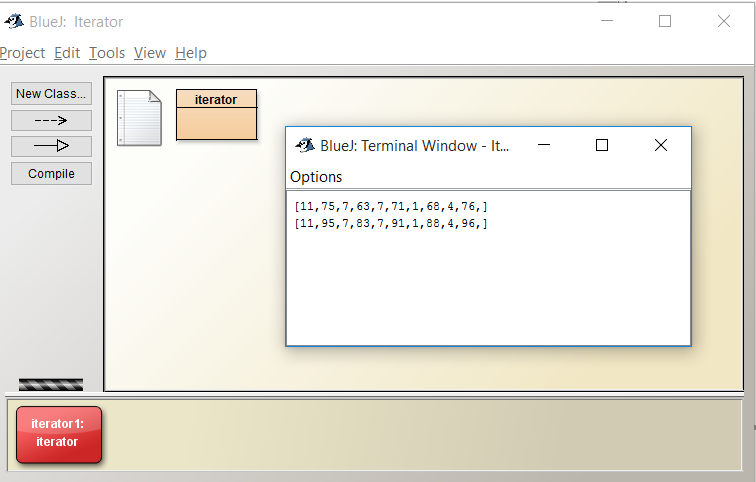
\includegraphics[scale=0.7]{./pics/bluej_iterator_code}
      \caption{Output for Iterator}
      \label{fig:bluej_iterator_code} 
\end{figure}

\subsection{Fibonacci}
The Fibonacci sequence in BlueJ can be expressed both by using an iterative and recursive approaches. An example can be seen in \figref{fig:bluej_fibo_code2}, where the user is prompted to give a number and the respective result is shown.

\begin{figure}[!h]
  \centering
    \begin{subfigure}[b]{0.45\textwidth}
    \begin{center}
      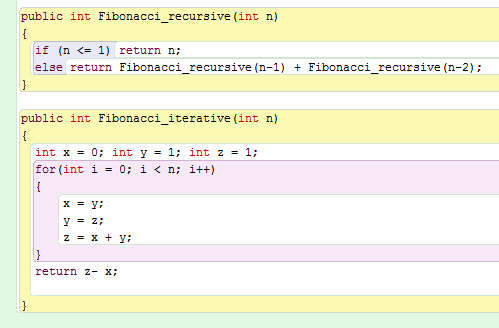
\includegraphics[scale=0.7]{./pics/bluej_fibo_code}
      \caption{BlueJ Fibonacci code.}
      \label{fig:bluej_fibo_code}
    \end{center}
    \end{subfigure}
    ~
    \begin{subfigure}[b]{0.45\textwidth}
    \begin{center}
      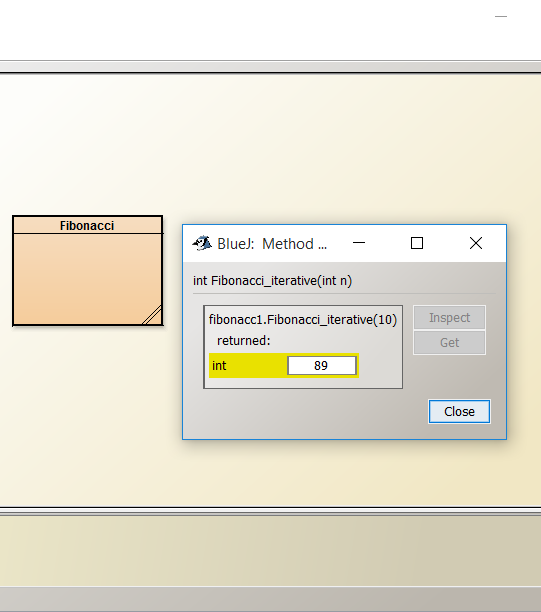
\includegraphics[scale=0.6]{./pics/bluej_fibo_code2}
      \caption{BlueJ Fibonacci output.}
      \label{fig:bluej_fibo_code2}
    \end{center}
    \end{subfigure}
    \caption{Code and output for Fibonacci numbers.}
    \label{fig:bluej_fibo}
\end{figure}
\subsection{Cups and Ball}
Similarly to how this game was implemented in Scratch, it gives the player the chance to guess where a ball might be among 15 identical cups, with the difference that it feels less intuitive since there is no visual feedback given but rather textual one - that the player has either successfully guessed the position of the ball or not. The code for \todo{watever chosen}, the class hierarchy and the final output can be seen in \figref{fig:bluej_ballcup_code}.

\begin{figure}[!h]
  \centering
      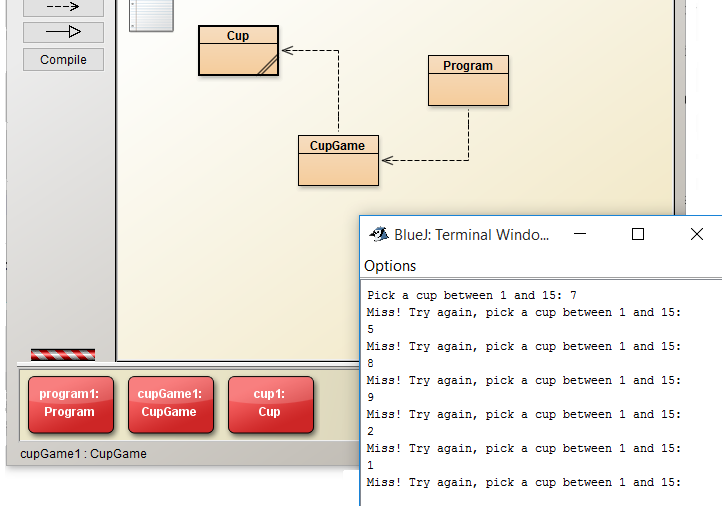
\includegraphics[scale=0.7]{./pics/bluej_ballcup_code}
      \caption{Output for Cups and Ball}
      \label{fig:bluej_ballcup_code} 
\end{figure}

\subsection{Hangman}
The Hangman is also a guessing game where the player has to guess a particular word by providing one letter at the time. In the BlueJ implementation, if the letter is part of the word, then it is added to a list of correct guesses. If not, it is added to a list of wrong guesses instead. Every time the player guesses a wrong letter, one of their lives is lost, thus the \lstinline!lives! counter decrements by one. If the player is to lose all of them eventually, the game is lost. The code follows an imperative style of programming with conditional statements and loops, some of which are shown on \figref{fig:bluej_hangman_code} 

\begin{figure}[!h]
  \centering
      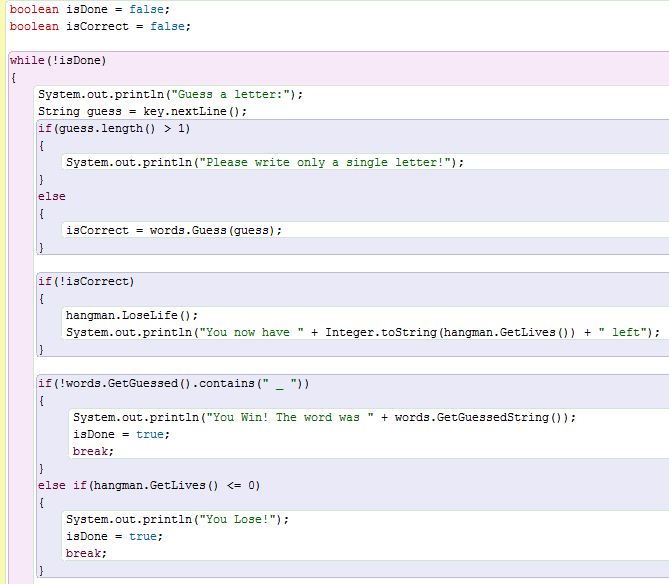
\includegraphics[scale=0.7]{./pics/bluej_hangman_code}
      \caption{Code for Hangman game}
      \label{fig:bluej_hangman_code} 
\end{figure}

\subsection{Criteria Evaluation}
\begin{description}[style=nextline]
\item[Readability]
BlueJ has reasonably good readability both by its textual and visual representations. The Main panel provides an overview of the hierarchy and interactions between different classes and objects. This gives novice programmers a greater understanding of how different pieces of the code are connected. Additionally, the textual representation provides good indentation and different colour schemes for every method so it is easier to understand the structure of the code.
\item[Writability]
As already mentioned in Section \ref{sec:bluej}, BlueJ uses Java as its underlying language. Writing code follows an object-oriented fashion and additionally keywords are highlighted in order to be differentiated by the programmer more easily.
\item[Observability]
BlueJ has fairly good observability as it usually manages to quickly and efficiently compile code. Additionally, single classes can be compiled separately in order to check their correctness. BlueJ's visual representation provides the option to create instances of objects as visual elements and call different methods specific to these objects in an easy, fast and understandable way. Problematic and erroneous sections are highlighted in red with an appropriate message for specific errors.  
\item[Trialability]
In terms of trialability, BlueJ has a good handling of syntactical and semantic errors. Where need be, exceptions are thrown and the code cannot be compiled before those are fixed. When a piece of code is compiled, if there is an error, the screen jumps to the specific location for the error, with an appropriate error message.
\item[Learnability]
BlueJ is first and foremost an educational platform, and it provides an intuitive interface, with a graphical representation of classes and objects. The intuitiveness is found in the possibility of creating and manipulating these through the Main panel.
\item[Reusability]
BlueJ uses the established practices for reusing code from Java such as class hierarchy, polymorphism etc.
\item[Pedagogic Value]
BlueJ is a powerful educational tool which provides a gentle introduction for novice programmers to the world of object-oriented programming.  BlueJ gives the option to visually create instances of classes and objects and playing around with their properties, giving the user a better understanding of how their hierarchical structure works. This is supplemented by its thorough documentation and exercises with steadily increasing difficulty.
\item[Environment]
Usually, the Integrated Development Environment (IDE) of a language is the only direct way of communication with that language. In the case of BlueJ, it provides the essentials needed for learning object orientation, specifically targeting novice programmers without the unnecessary clutter present in more advanced IDEs such as Eclipse or NetBeans. Furthermore, it does not require much effort to install it and create projects in it.
\item[Documentation]
As already mentioned, BlueJ has a solid documentation with a lot of reference materials and additional exercises for those who are interested to delve deeper in its features. Also it is fairly easy to get access to the documentation on the BlueJ homepage without the need for any additional books. Furthermore, all of the documentation meant for Java is also applicable for BlueJ.
\item[Uniformity]
BlueJ has a high uniformity compared to other languages since Java is one of the mainstream general purpose languages, to which other languages compare their uniformity.
\end{description}